\documentclass[12pt]{book}
\usepackage{amsmath}
\usepackage{float}
\usepackage[margin=1.5in]{geometry}
\usepackage{enumitem}
\usepackage{xcolor}
\usepackage{cancel}
\usepackage{graphicx}



\title{Introduction to Mechanics}
\author{Nathan Butcher}

\begin{document}
\graphicspath{{Figures/Units} {Figures/Forces}}
\newcounter{chp}
\setcounter{chp}{0}
\newcounter{example}

\newcommand{\scinot}[2]{#1 \cdot 10^{#2}}

%Start a new example using counters
\newcommand{\example}{\textbf{Example \texttt{\thechp}.\texttt{\theexample}}
\addtocounter{example}{1}

\hspace{10pt}
}

%Give a horizontal line with space to separte things
%like examples or asides
\newcommand{\linespace}{\hspace{10pt}

\hrule

\hspace{10pt}}

\newenvironment{exampleblock}
{
\linespace

\example

}
{

\linespace

}

\chapter{Introduction, Numbers, and Units}

\setcounter{example}{1}
\addtocounter{chp}{1}

In physics we study the interactions and motion of matter. For our introduction in this class, we will mostly study what I like to call ``Physics at the human scale'' because it is the physics of daily life that we observe and directly interact with. It describes an apple falling from a tree, a car slamming its brakes, a pendulum swinging, the collision of 2 billiard balls, and more.

\section{Math and scientific notation}

This text will assume that you are comfortable with using algebra to solve an equation for a variable and that you have had a class on trigonometry. We will review those topics as they come up but it may be difficult to follow without the math background.

During this text we will use \textbf{scientific notation} frequently to write very large or very small numbers in an easier to read format. With it, we write a number in the format

\begin{equation}
\scinot{a}{b}
\end{equation}

where $1 \leq a < 10$ and $b$ is an integer. This saves us from having to write and count a lot of zeros that indicate place. The number is a factor multiplied by a power of 10.

\begin{exampleblock}

Write the number 38,500,000 in scientific notation.

\hspace{10pt}

To write this in the form $\scinot{a}{b}$, first let's find $a$ such that $1 \leq a < 10$. Since our number starts with the digits 385, that means $a = 3.85$. From here we have

\begin{equation}
38,500,000 = 3.85 \cdot 10,000,000
\end{equation}

Now we need to write 10,000,000 as a power of 10. There are 7 zeros, so it will be $10^7$. This means that our number is 

\begin{equation}
\scinot{3.85}{7}
\end{equation}

\end{exampleblock}

\begin{exampleblock}

Write the number 0.000007018 in scientific notation.

\hspace{10pt}

We can use the same reasoning as the above example to find that $a = 7.018$. The number can be written as

\begin{equation}
0.000007018 = 7.018 \cdot 0.000001
\end{equation}

Now we just need to find the power of 10. Let's start looking at powers of 10.

\begin{equation}
\begin{split}
10^0 = 1 \\
10^{-1} = \frac{1}{10} = 0.1 \\
10^{-2} = \frac{1}{10^2} = 0.01 \\
10^{-3} = \frac{1}{10^3} = 0.001
\end{split}
\end{equation}

A negative power means to take 1 divided by the number to that positive power. Looking at 10, we see that as we decrease the power (larger negative value), we move the decimal point 1 to the left. This will give us

\begin{equation}
0.000001 = \frac{1}{10^6} = 10^{-6}
\end{equation}

which makes our number

\begin{equation}
0.000007018 = \scinot{7.018}{-6}
\end{equation}

\end{exampleblock}

\section{Units}

Physicists will try to describe the world around us quantitatively, meaning with numbers. In order to ascribe meaning to those numbers we need to use physical \textbf{units}. For example, think about if you were baking a loaf of bread and the recipe called for ``4 flour''. Would you know how much flour was required? The recipe should say ``4 \textit{cups} of flour'' so that you know the amount required for the bread. 

In physics, like most sciences, we use \textbf{SI units}. In the USA, you likely encounter the Imperial system of units in daily life. Common Imperial units you might have seen include the inch for length and gallon for volume. These units are not the standard for scientific disciplines, and as such we will focus on using SI units. There are 3 base units that we will use frequently:

\begin{itemize}
\item \textbf{kilogram} - the SI base unit of mass. Mass is a measure of how much matter there is. It is related to but not the same as weight. We will discuss weight further in a later chapter, but for now think of mass as how much ``stuff'' there is.

\item \textbf{meter} - the SI base unit of length. If you don't have a good mental picture of a meter, it is a little longer than 3 feet.

\item \textbf{second} - the SI base unit of time. We will continue to see minutes and hours used throughout, but for doing quantitative work we will want to use seconds for everything.
\end{itemize}

\section{SI Prefixes}

With these SI base units we use \textbf{prefixes} to scale the units relative to our problem. Table \ref{SIPrefixes} contains several of the most common prefixes, with the bolded ones being most important for this class.

\begin{table}[b]
\large
\centering
\caption{SI Prefixes}
\begin{tabular}{ c | c | c }
	\hline
	Prefix & Abbreviation & Numerical value \\
	\hline
	nano- & n & $10^{-9}$ \\
	micro- & $\mu$ (Greek letter \textit{mu}) & $10^{-6}$ \\
	\textbf{milli-} & m & $10^{-3}$ \\
	\textbf{centi-} & c & $10^{-2}$ \\
	\textbf{kilo-} & k & $10^3$ \\
	mega- & M & $10^6$ \\
	giga- & G & $10^9$ \\
	\hline
\end{tabular}

\label{SIPrefixes}
\end{table}

One thing you should see is that SI prefixes allow us to scale our units by powers of 10. This is much simpler than the Imperial system. For lengths we have 12 inches to a foot, 3 feet to a yard, and 1760 yards to a mile. Compare this to just multiplying or dividing by powers of 10 and see how much simpler SI units are to work with!

The main purpose to having the prefixes is it allows us to scale the units to our problem. If we were to talk about the distance between San Diego and Los Angeles, it would make sense to use kilometers because that distance is about 194 kilometers. In meters, it would be $194 \cdot 10^3 = 194,000$ meters. Prefixes allow us to use numbers that are closer to 1, which are easier to read and for our brains to process. 

There are other prefixes and units that are used within different branches of physics and other fields of science. We will see some of this in CHAPTER HERE when we discuss the solar system. Again, the goal is always to make the numbers we work with closer to 1.

In addition to the base units, we will also have \textbf{derived units}, which are a combination of SI base units. On a car speedometer you may have seen the unit $km/hr$, which means ``kilometers per hour''. This is a derived unit because it combines the units of length and time.


\section{Converting units}

Now that we have SI prefixes, it is important that we learn how to convert between different units. This process is called \textbf{dimensional analysis} because the units are the ``dimensions'' that we are looking at.

To convert units, we will write unit factors that are fractions equal to 1. For example, 

\begin{equation}
\frac{1 \, mm}{10^{-3} \, m} = 1
\end{equation}

is a unit factor that equals 1 because the prefix milli- means $10^{-3}$, so 1 millimeter is equal to $10^{-3}$ meter. This fraction can by multiplied by a quantity to change the unit but not the physical value because the fraction is 1. Now lets use that to convert 3.25 meters to millimeters. We can use the unit fraction to cancel the meters from the original value, and have a unit of millimeters left in the numerator.

\begin{equation}
3.25 \, \cancel{m} \cdot \frac{1 \, mm}{10^{-3} \, \cancel{m}} = 3,250 \, mm
\end{equation}


The reason this works is that our unit fraction is equal to 1, so multiplying our original quantity by that unit fraction doesn't change the value! It only changes what unit that value is given in.

You could also think of the unit fraction as 1,000 millimeters in a meter.

\begin{equation}
3.25 \, \cancel{m} \cdot \frac{1000 \, mm}{1 \, \cancel{m}} = 3,250 \, mm
\end{equation}

Both $\frac{1000 \, mm}{1 \, m}$ and $\frac{1 \, mm}{10^{-3} \, m}$ are valid unit fractions for converting from meters to millieters. They are equally correct, so use whichever you prefer!

%\textbf{Example \texttt{\thechp}.\texttt{\theexample}}
%\addtocounter{example}{1}
\begin{exampleblock}

\textbf{Convert 500 nanometers to centimeters.}

\hspace{10pt}

We can convert 500 nanometers to meters first, then convert from meters to centimeters.

\begin{equation}
500 \, \cancel{nm} \cdot = \frac{10^{-9} \, m}{1 \, \cancel{nm}} = 5 \cdot 10^{-7} \, m
\end{equation}

\begin{equation}
\scinot{5}{-7} \, \cancel{m} = \frac{100 \, cm}{1 \, \cancel{m}} = \scinot{5}{-5} \, cm 
\end{equation}

Sometimes it is useful to convert to an intermediary unit to help you get to the requested final unit.
\end{exampleblock}

%\linespace

%\example

\begin{exampleblock}

Convert 1 meter to feet. Use the following information:

\begin{itemize}
\item 1 foot = 12 inches
\item 1 inch = 2.54 cm
\end{itemize}

The given unit conversions tell us how to solve this problem. First we convert the meter to centimeters, then use the given conversion from centimeters to inches. Finally, we can use the given conversion from inches to feet.

\begin{equation}
1 \, \cancel{m} \cdot \frac{100 \, \cancel{cm}}{1 \, \cancel{m}} \cdot \frac{1 \, \cancel{in}}{2.54 \, \cancel{cm}} \cdot \frac{1 \, foot}{12 \, \cancel{in}} = 3.28 \, feet
\end{equation}

\end{exampleblock}

\begin{exampleblock}

A car is driving at 45 kilometers per hour $\frac{km}{hr}$. Convert this to meters per second $\frac{m}{s}$

\hspace{10pt}

First let's write out the unit to help us see how to convert this.

\begin{equation}
45 \, \frac{km}{hr}
\end{equation}

This means that the car moves 45 kilometers in 1 hour. When doing unit conversions it may be helpful to write out the unit like that

\begin{equation}
45 \, \frac{km}{hr} = \frac{45 \, km}{1 \, hr}
\end{equation}

We have kilometers in the numerator and hours in the denominator, so we have to make sure we write our unit fractions correctly to cancel them. First, let's convert the kilometers to meters.

\begin{equation}
\frac{45 \, \cancel{km}}{1 \, hr} \cdot \frac{10^3 \, m}{1 \, \cancel{km}} = \frac{45,000 \, m}{1 \, hr}
\end{equation}

Now we can convert the hour to seconds. It may be helpful to convert to minutes first, then to seconds.

\begin{equation}
\frac{45,000 \, m}{1 \, \cancel{hr}} \cdot \frac{1 \, \cancel{hr}}{60 \, \cancel{min}} \cdot \frac{1 \, \cancel{min}}{60 \, s} = \frac{12.5 \, m}{1 \, s}
\end{equation}

The car is driving at $12.5 \, \frac{m}{s}$.

\end{exampleblock}

\chapter{Quantities of motion and kinematics}
\setcounter{example}{1}
\addtocounter{chp}{1}

The first thing we must do to describe the motion of objects is define specific terms that we will use. These terms will have clear, specific definitions that may differ from how they are used in everyday language. 

\section{Motion definitions}

The first quantity to talk about is \textbf{position}. This is a measurement of where something is along an axis (or multiple axes). This is a length, so the SI unit for position is the meter. Position will be denoted with the variable $x$ in equations.

When we study motion, we often look at an object moving from one position to the other. The first position is the \textbf{initial} position, and the second position is the \textbf{final} position. In equations we will use subscript $i$ and $f$ for initial final respectively, so that the initial position is $x_i$ and the final position is $x_f$. To indicate the change in a quantity we will use $\Delta$, which is the Greek letter Delta. The change in position between the initial state and final state can be written as

\begin{equation}
\Delta x = x_f - x_i
\end{equation}

which is a measure of how the position changed moving from the initial state $x_i$ to the final state $x_f$. 

The second quantity we will talk about is \textbf{velocity}. This is a measurement of the rate of change in position of a moving object.  Velocity will be denoted with the variable $v$ in equations. Velocity has a direction, so it is a vector quantity. The direction can be denoted with a positive or negative sign to indicate the direction along a position axis.

\textbf{Average velocity} is the average rate of change in position as an object moves from its initial position $x_i$ to its final position $x_f$ over a time interval $\Delta t$. For average velocity we will use a subscript ``avg'', so it is written as $v_{avg}$. 

\begin{equation}
v_{avg} = \frac{\Delta x}{\Delta t}
\end{equation}

Average velocity does not give us any information about the moment-to-moment velocity throughout the motion, only the average throughout the time interval.

From the equation above, we see that velocity is a length divided by time. This means our SI unit is $\frac{m}{s}$ , which is read as \textit{meters per second}. 

The third quantity we will talk about is \textbf{acceleration}. This is a measurement of the rate of change of velocity of a moving object. Acceleration will be denoted with the variable $a$ in equations. Acceleration has a direction, so it is a vector quantity. 

\textbf{Average acceleration} is the average rate of change in velocity as an object moves from its initial position $x_i$ to its final position $x_f$ over a time interval $\Delta t$. Similar to position, the initial velocity is $v_i$, the final velocity is $v_f$, and the change in velocity is $\Delta v = v_f - v_i$.

\begin{equation}
a_{avg} = \frac{\Delta v}{\Delta t}
\end{equation}

Again, average acceleration gives us the average value over the entire interval of motion but no information about the moment-to-moment value of the acceleration.

From the equation above, we see that acceleration is a velocity divided by time. Our SI unit is $\frac{m/s}{s}$, which is read as \textit{meters per second per second}. The unit can also be written as $\frac{m}{s^2}$, which is read as \textit{meters per second squared}. These two ways of writing the units of acceleration are equivalent and both are correct. For the rest of this text, I will use $\frac{m}{s^2}$.

\begin{exampleblock}

Alice starts at a position of $2.0 \, m$ and walks to a position of $6.0 \, m$ over a duration of $8.0 \, s$. What is her average velocity while she is walking?

\begin{figure}[h]
\centering
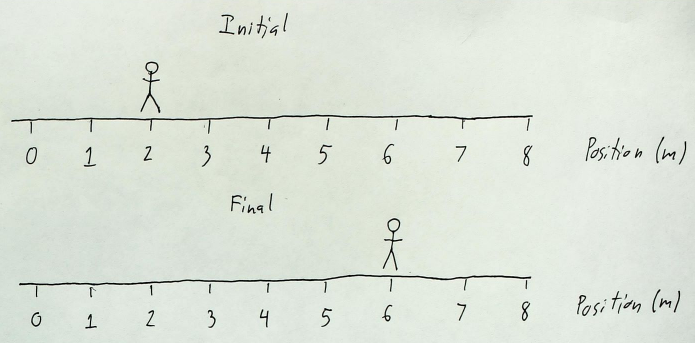
\includegraphics[scale=0.8]{example_units_velocity_walking.png}
\end{figure}

We know Alice's initial position $x_i = 2.0 \, m$ and final position $x_f = 6.0 \, m$. This means her change in position is

\begin{equation}
\Delta x = x_f - x_i
\end{equation}

\begin{equation}
\Delta x = 6.0 \, m - 2.0 \, m = 4.0 \, m
\end{equation}

In the problem we are told she walks for $8.0 \, s$, so our time duration is $\Delta t = 8.0 \, s$. Now we can use the definition of average velocity

\begin{equation}
v_{avg} = \frac{\Delta x}{\Delta t}
\end{equation}

\begin{equation}
v_{avg} = \frac{4.0 \, m}{8.0 \, s} = 0.50 \, \frac{m}{s}
\end{equation}

Her average velocity is $0.50 \, \frac{m}{s}$. Notice how we get the units of $\frac{m}{s}$ by just dividing the units in the equation.

\end{exampleblock}

The final quantity we will introduce is \textbf{speed}. This is a measurement of how fast an object is moving. You might be familiar with miles per hour (mph) or kilometers per hour ($\frac{km}{hr}$) from a car speedometer. The SI unit of speed is $\frac{m}{s}$, same as velocity. Speed will be denoted as $s$ in equations.

\textbf{Average speed} can be found by taking the distance traveled $d$ over the time duration $\Delta t$.

\begin{equation}
s_{avg} = \frac{d}{\Delta t}
\end{equation}

One important issue we must address is how average speed differs from average velocity. Both are measured in units of $\frac{m}{s}$ and can be used to get information about how fast an object moved.

\begin{enumerate}
\item Speed is a scalar quantity, not a vector quantity. Speed does not tell you anything about the direction of motion. There is no such thing as a negative speed because the distance traveled will always be zero or positive.

\item The distance traveled is not always the same as the change in position. Velocity only depends on $x_i$, $x_f$, and $\Delta t$ with no concern for the path taken between $x_i$ and $x_f$. Speed depends on the distance traveled so it does matter what the path taken is.
\end{enumerate}

The last new definitions we will introduce here are \textbf{instantaneous speed} and \textbf{instantaneous velocity}. Instantaneous speed is a measure of the speed at an instant in time. Instantaneous velocity is the rate of change in position at an instant in time, which can also be thought of as the instantaneous speed plus the direction of travel.

\section{Motion Graphs}

One helpful tool for studying the motion of objects is to use graphs. This allows us to present data in a visual format rather than text. The x-axis will be the time and the y-axis will be position, velocity, or acceleration.

First, let's start with the following graph of position vs. time (which is also called an \textit{x vs t} plot).

\begin{figure}[H]
\centering
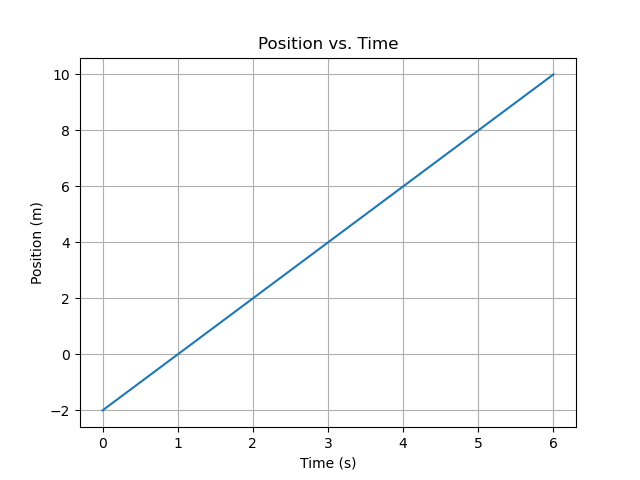
\includegraphics[scale=0.6]{position1.png}
\caption{Sample position vs. time graph}
\label{pos1}
\end{figure}

The graph has a title that tells you what the graph shows and the x- and y-axes are labeled, including units. These features are important to allow somebody reading your graph to easily understand what it is showing. 

This graph has time in seconds on the x-axis and position in meters on the y-axis. What this graph is showing is therefore the position of an object as it moves over time. For example, if we wanted to find the position of the object at $t = 4 \, s$ we would look at the y-value of the graph at $4 \, s$. The position of the object is therefore $x = 6 \, m$.

What if we wanted to find the average velocity of the object throughout this motion? It moves for 6 seconds, so $\Delta t = 6 \, s$. The position at $t = 0 \, s$ is $x = -2 \, m$, so we have in the initial state $x_i = -2 \, m$. The position at $t = 6 \, s$ is $x = 10 \, m$, so we have in the final state $x_f = 10 \, m$.

\begin{equation}
v_{avg} = \frac{\Delta x}{\Delta t} = \frac{10 \, m - (-2) \, m}{6 \, s} = 2 \, \frac{m}{s}
\end{equation}

Since our y-value is position and x-value is time, what we just did above is find the slope of the line! We can extend this in general to recognize that \textbf{the slope of a \textit{x vs t} graph is the velocity.} We can use this to find instantaneous velocities by finding the slope at a point on the graph! Below is a plot of velocity vs. time that describes the same motion.

\begin{figure}[H]
\centering
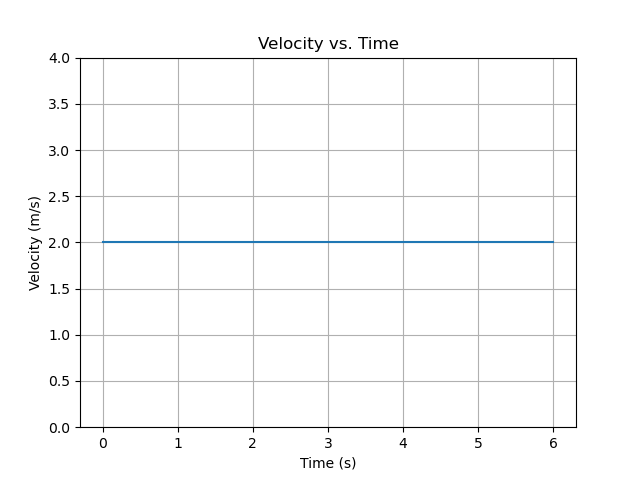
\includegraphics[scale=0.6]{velocity1.png}
\caption{Sample velocity vs. time graph for the same motion as \ref{pos1}.}
\end{figure}

The slope of the \textit{x vs t} plot is constant, so the velocity doesn't change throughout the motion. From $0 \, s$ to $6 \, s$ we have $v = 2 \, \frac{m}{s}$. Next lets look at what we call the ``area under the curve'', which is the area of the graph between the x-axis and the graph value. Since the velocity is constant, the area is just a rectangle

\begin{equation}
Area = 2.0 \, \frac{m}{s} \cdot 6 \, s = 12 \, m
\end{equation}

Back to the \textit{x vs t} plot where we had $x_f = 10 \, m$ and $x_i = -2 \, m$, we have a change in position

\begin{equation}
\Delta x = x_f - x_i = 10 \, m - (-2) \, m = 12 \, m
\end{equation}

\textbf{The area under the graph of a \textit{v vs t} graph is the change in position of the object!} Since the y-axis is velocity and the x-axis is time, we are multiplying the velocity by the time to get the change in position. Note that the \textit{v vs t} graph does not tell us what the value of $x_i$ is, just how much the position changes by.


This is a good time to make a very important point: \textbf{motion graphs are not a ``picture'' of the motion, but instead a visual representation of data}. The \textit{x vs t} and \textit{v vs t} look very different from each other despite describing the same motion. That is because they show how the position and velocity change over time, not provide a ``picture'' of how the object moves. In almost every case the position, velocity, and acceleration graphs for a moving object will all look very different from each other.

Using the same rational as above, the acceleration is the slope of the \textit{v vs t} graph and the change in velocity is the area under the \textit{a vs t} graph. We will try these concepts out in the example below.

\begin{exampleblock}

The acceleration of an object over time is measured as

\begin{table}[h]
\large
\centering
\caption{Acceleration vs Time example}
\begin{tabular}{| c | c |}
	\hline
	Time ($s$) & Acceleration ($m/s^2$) \\
	\hline
	0 & 9 \\ \hline
	1 & 7 \\ \hline
	2 & 5 \\ \hline
	3 & 3 \\ \hline
	4 & 1 \\ 
	\hline
\end{tabular}
\label{atable_ex1}
\end{table}

\begin{enumerate}
\item Plot the acceleration vs. time.
\item Use the acceleration vs. time graph to create a velocity vs. time graph if the velocity at $t = 0 \, s$ is $v = -4 \, m/s$.
\end{enumerate}

First we can create our \textit{a vs. t} plot with time on the x-axis and acceleration on the y-axis. We can see the plot in \ref{atable_motiongraph_ex1}, where the data points have been plotted and fit with a line.

\begin{figure}[h]
\centering
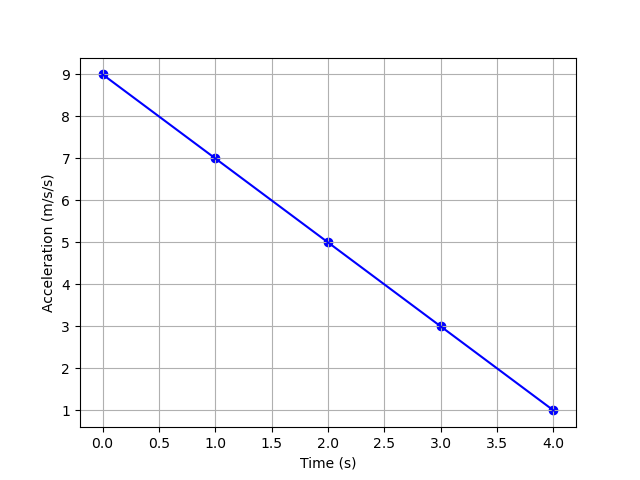
\includegraphics[scale=0.6]{example_accel.png}
\caption{Graph created from data in \ref{atable_ex1}}
\label{atable_motiongraph_ex1}
\end{figure}

We see that the acceleration changes linearly (as a straight line) with time. The acceleration is positive and decreasing over the entire duration of the graph.

Now we can use the \textit{a vs. t} graph to create our \textit{v vs. t} graph. The change in velocity over time is the area under the curve of the \textit{a vs. t} graph. With the acceleration changing over time, how can we find the area under the curve?

Let's focus first on the interval $t = 0 \, s$ to $t = 1 \, s$. The acceleration is linear, so the average acceleration over the interval is 

\begin{equation}
a_{avg} = \frac{a(t=0) + a(t=1)}{2}
\end{equation}

The acceleration is a function of time, so $a(t=0)$ means the acceleration at $t = 0 \, s$ and $a(t=1)$ means the acceleration at $t = 1 \, s$. The average acceleration between $t = 0 \, s$ and $t = 1 \, s$ is

\begin{equation}
a_{avg} = \frac{9 \, m/s^2 + 7 \, m/s^2}{2} = 8 \, \frac{m}{s^2}
\end{equation}

The area under the curve is the average acceleration multiplied by the time, which is $1 \, s$ for this interval

\begin{equation}
\Delta v = a_{avg} \cdot \Delta t
\end{equation}

\begin{equation}
\Delta v = (8 \, \frac{m}{s^2}) (1 \, s) = 8 \, \frac{m}{s}
\end{equation}

The velocity at $t = 1 \, s$ is the velocity at $t = 0 \, s$ plus the change in velocity between $t = 0 \, s$ and $t = 1 \, s$.

\begin{equation}
v(t=1) = v(t=0) + \Delta v
\end{equation}

\begin{equation}
v(t=1) = -4 \, \frac{m}{s} + 8 \, \frac{m}{s} = 4 \, \frac{m}{s}
\end{equation}

Try repeating this process for each one second interval. The velocities that you should get are shown in \ref{vtable_ex1}.

\begin{table}[h]
\large
\centering
\caption{Velocity vs Time example}
\begin{tabular}{| c | c |}
	\hline
	Time ($s$) & Velocity ($m/s$) \\
	\hline
	0 & -4 \\ \hline
	1 & 4 \\ \hline
	2 & 10 \\ \hline
	3 & 14 \\ \hline
	4 & 16 \\ 
	\hline
\end{tabular}
\label{vtable_ex1}
\end{table}



\begin{figure}[h]
\centering
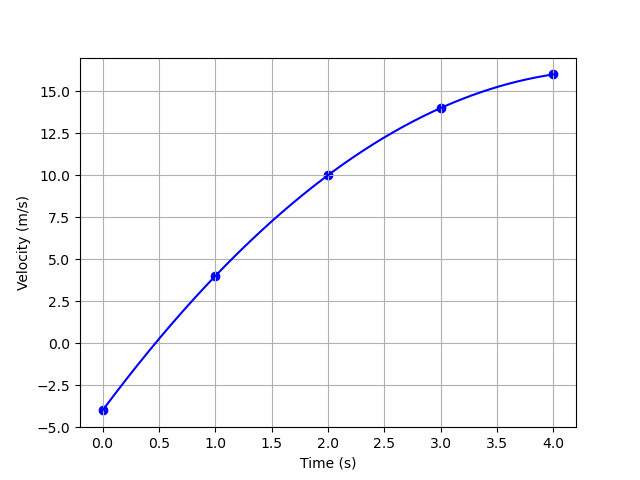
\includegraphics[scale=0.6]{example_vel.png}
\caption{Velocity vs time graph created from the data in \ref{atable_ex1} and initial condition of $v = -4 \frac{m}{s}$ at $t = 0 \, s$.}
\end{figure}

This graph is a parabola which opens downward. If you are taking or have taken calculus, you would recognize this as being the integral of the \textit{a vs. t} graph. 

\end{exampleblock}

\newpage

\section{Constant acceleration motion}

One case of particular interest we will look at is \textbf{constant acceleration motion}, where the acceleration does not change over an interval of time. This is useful for 2 reasons:

\begin{enumerate}
\item Common. There are several examples of constant acceleration motion or motion that is close enough to having a constant acceleration that we can approximate it as such. This gives us a useful way to describe a variety of physical situations.

\item Easy to work with mathematically.
\end{enumerate}

We will start by saying that acceleration is constant as a function of time

\begin{equation}
\begin{split}
a(t) = a \\
a_i = a_f = a
\end{split}
\end{equation}

Now we will consider motion from a time of zero ($t = 0 \, s$) to some later time $t$. This means that our $\Delta t$ is

\begin{equation}
\Delta t = t - 0 = t
\end{equation}

Now we can work with our definition of average acceleration. If the acceleration is constant, then the average acceleration is the constant value of acceleration $a_{avg} = a$. Let's see if we can find the velocity $v_f$ at a time $t$ starting with the definition of acceleration.

\begin{equation}
a = \frac{\Delta v}{\Delta t}
\end{equation}

\begin{equation}
a = \frac{v_f - v_0}{t}
\end{equation}

Above we see a subscript zero for the first time. The variable $v_0$ is pronounced ``v naught'' and is used to indicated the value of a motion variable at time zero. It is the special case of the initial state being at time zero.

Continuing on with the equation, we can multiply both sides by $t$.

\begin{equation}
at = v_f - v_0
\end{equation}

Now we can add $v_0$ to both sides to get.

\begin{equation}
v_f = v_0 + at
\label{km1}
\end{equation}

Which gives us the final velocity $v_f$ at a time $t$ given the velocity at $t = 0 \, s$ is $v_0$ and the acceleration is a constant value of $a$. This is the first of the \textbf{kinematic equations}, which are used to describe constant acceleration motion.

Constant acceleration motion has a linear velocity, which means we can find the average velocity as 

\begin{equation}
v_{avg} = \frac{v_0 + v_f}{2}
\label{kmvavg1}
\end{equation}

From the definition of average velocity, we also have 

\begin{equation}
v_{avg} = \frac{\Delta x}{t}
\label{kmvavg2}
\end{equation}


Now we can set the right hand sides of \ref{kmvavg1} and \ref{kmvavg2} equal and solve for $\Delta x$

\begin{equation}
\frac{\Delta x}{t} = \frac{v_0 + v_f}{2}
\end{equation}

\begin{equation}
\Delta x = \frac{v_0 + v_f}{2} \cdot t
\label{km2}
\end{equation}

This is the second kinematic equation, used for finding the change in position if we know the initial and final velocities. We can get a third kinematic equation that does not include $v_f$ if we use the definition of $v_f$ from equation \ref{km1} and plug that into equation \ref{km2}.

\begin{equation}
\Delta x = \frac{v_0 + v_0 + at}{2} \cdot t
\end{equation}

\begin{equation}
x_f - x_0 =  (v_0 + \frac{1}{2}at) \cdot t
\end{equation}

\begin{equation}
x_f = x_0 + v_0 t + \frac{1}{2} a t^2
\label{km3}
\end{equation}

This is the third kinematic equation and gives us the final position as a function of initial quantities.

So far, these 3 kinematic equations have all included time as a variable. What if we don't know or care about the time but want to study how other quantities are related. Let's return to \ref{km1} and solve for time $t$.

\begin{equation}
v_f = v_0 + at
\end{equation}

\begin{equation}
v_f - v_0 = at
\end{equation}

\begin{equation}
t = \frac{v_f - v_0}{a}
\end{equation}

Now we can take this expression for $t$ and plug it into \ref{km3}.

\begin{equation}
x_f = x_0 + v_0 \left( \frac{v_f - v_0}{a} \right) + \frac{1}{2} a \left( \frac{v_f - v_0}{a} \right)^2
\end{equation}

We can simplify by moving $x_0$ and working with the terms in parentheses.

\begin{equation}
x_f - x_0 = \frac{1}{a} (v_f v_0 - v_0^2) + \frac{1}{2}a \left( \frac{v_f^2 - 2 v_f v_0 + v_0^2}{a^2} \right)
\end{equation}

This may look like a mess but don't worry, we will get a nice equation when we are done. We will replace $x_f - x_0$ with $\Delta x$, since that is the definition of the change in position. Also, we will simplify the second term on the right hand side by distributing the $\frac{1}{2}$ and pulling $\frac{1}{a^2}$ out of the parentheses.

\begin{equation}
\Delta x = \frac{1}{a} (v_f v_0 - v_0^2) + \frac{1}{a} (\frac{1}{2} v_f^2 - v_f v_0 + \frac{1}{2} v_0^2)
\end{equation}

If we multiply both sides by $a$, we can remove the parentheses and group the like terms on the right hand side.

\begin{equation}
a \Delta x = v_f v_0 - v_0^2 + \frac{1}{2} v_f^2 - v_f v_0 + \frac{1}{2} v_0^2
\end{equation}

\begin{equation}
a \Delta x = \frac{1}{2} v_f^2 + v_f v_0 - v_f v_0 + \frac{1}{2} v_0^2 - v_0^2
\end{equation}

The $v_f v_0$ cross terms actually cancel out!

\begin{equation}
a \Delta x = \frac{1}{2} v_f^2 - \frac{1}{2} v_0^2
\end{equation}

Now we can solve this equation for $v_f^2$.

\begin{equation}
2 a \Delta x	 = v_f^2 - v_0^2
\end{equation}

\begin{equation}
v_f^2 = v_0^2 + 2 a \Delta x
\label{km4}
\end{equation}

Here we have the fourth kinematic equation, which does not include time but instead the change in position, initial velocity, final velocity, and acceleration.

All of the equations are collected in \ref{kmtable}. When presented with a problem, looking at what variable each kinematic equation is missing can help you choose what equation to use. We will go through a few examples and walk through problem solving in more detail. Throughout studying motion with kinematic equations, you need to remember that \textbf{we can only use the kinematic equations with constant acceleration motion}. We derived these equations from the starting point of constant acceleration, so if acceleration changes then these equations are no longer valid. 

\begin{table}[b]
\large
\centering
\caption{Kinematic Equation}
\label{kmtable}
\begin{tabular}{| c | c | c |}
	\hline
	Equation number & Formula & Missing variable \\
	\hline
	1 & $v_f = v_0 + at$ & No position \\[5pt] \hline
	2 & $\Delta x = \frac{v_0 + v_f}{2} \cdot t$ & No acceleration \\[5pt] \hline
	3 & $x_f = x_0 + v_0 t + \frac{1}{2} a t^2$ & No final velocity \\[5pt] \hline
	4 & $v_f^2 = v_0^2 + 2 a \Delta x$ & No time \\[5pt]
	\hline
\end{tabular}
\end{table}

\newpage

\section{Problem solving with kinematic equations}

We can follow a basic outline to solving constant acceleration problems using kinematic equations. A typical problem will have a couple sentences describing a physical scenario and asking for a quantity of the motion. When approaching a problem, you should go use the following steps:

\begin{enumerate}
\item Identify the known quantities in the problem. This is the information the problem gives you. Drawing a picture is often useful!

\item Identify the quantity that we are trying to solve for.

\item Choose a kinematic equation that contains the known quantities and the one we wish to solve for.

\item Solve the kinematic equation algebraically for the quantity of motion we are trying to find. Do not plug in numbers before doing this!

\item Plug in numbers and solve the problem.
\end{enumerate}

It is important to not plug in numbers early because that makes it difficult to find any mistakes in the solution. Finding algebra mistakes with variables is much easier than finding mistakes with numbers.

\begin{exampleblock}

A ball rolling down a ramp accelerates at $3.0 \, m/s^2$. If the ramp is $L = 2.5 \, m$ long and the ball is released from rest at the top of the ramp, how what is the velocity of the ball when it reaches the bottom of the ramp?

\begin{figure}[h]
\centering
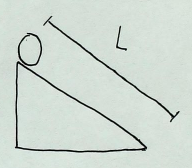
\includegraphics[scale=0.8]{example_units_ball_ramp.png}
\end{figure}

\hspace{10pt}

First we can take stock of what we know. We have the acceleration $a = 3.0 \, m/s^2$ given. The ball travels from the top to the bottom of the ramp, so the change in position is the length of the ramp $\Delta x = 2.5 \, m$. That may look like all of the given information, but there is one more thing we are given. The problem states that the ball ``is released from rest'', which means that the ball is stationary when the motion starts (``at rest'' means it is still or stationary). Therefore, we also know that $v_0 = 0 \, m/s$.

We want to solve for the velocity at the bottom of the ramp. This is the final state of the problem, so that is our final velocity $v_f$.

We don't have time, so it makes sense to look at the 4th kinematic equation.

\begin{equation}
v_f^2 = v_0^2 + 2 a \Delta x
\end{equation}

The only value we don't have here is $v_f$, so this will work. Let's take the square root of both sides to solve for velocity.

\begin{equation}
v_f = \sqrt{v_0^2 + 2 a \Delta x}
\end{equation}

Plug in numbers.

\begin{equation}
v_f = \sqrt{(0 \, m/s)^2 + 2 (3.0 \, m/s^2) (2.5 \, m)}
\end{equation}

\begin{equation}
v_f = \sqrt{15 \, m^2 / s^2} = 3.9 \, m/s
\end{equation}

The ball has a velocity of $3.9 \, m/s$ when it reaches the bottom of the ramp. Notice how tracking the units shows we get units of $m/s$ at the end to help us verify that our work was correct. This is why it is good to track units!

\end{exampleblock}

\begin{exampleblock}

A car that is driving at $34 \, m/s$ begins to brake, slowing down at an acceleration of $1.5 \, m/s^2$. If the car ends at a velocity of $28 \, m/s$, how much time was it slowing down for?

\hspace{10pt}

We know that the car starts at a velocity of $v_0 = 34.0 \, m/s$ and ends at a velocity of $v_f = 28.0 \, m/s$. The acceleration of the car is causing it to slow down, which means the acceleration is in the opposite direction as the velocity. Therefore, the acceleration is negative, with a value of $a = -1.5 \, m/s^2$.

We need to solve for the time $t$ that it takes to change from $v_0$ to $v_f$ with an acceleration $a$. This means we want to use the 1st kinematic equation.

\begin{equation}
v_f = v_0 + at
\end{equation}

Now we can solve this algebraically for $t$.

\begin{equation}
v_f - v_0 = at
\end{equation}

\begin{equation}
t = \frac{v_f - v_0}{a}
\end{equation}

Now we can plug in numbers

\begin{equation}
t = \frac{28.0 \, m/s - 34.0 \, m/s}{-1.5 \, m/s^2} = \frac{-6.0 \, m/s}{-1.5 \, m/s^2} = 4.0 \, s
\end{equation}

The car has to hit the brakes for $4.0 \, s$ to slow down as described in the problem. 

\end{exampleblock}

The general outline to problem solving here will be useful throughout your studies in physics. The variables and equations involved will change, but the method remains the same.

\section{Gravity and free-fall}
\label{gravsec}

One common scenario where we have constant acceleration is when an object is being acted on by gravity at the Earth's surface. At the Earth's surface, \textbf{gravity} causes an object to accelerate straight down toward to the center of the Earth. When an object is accelerating only due to gravity, we call that $free-fall$. Free-fall ignores other effects like air resistance (which we will talk about more later), so it works in cases where those effects are very small. An example is a thrown baseball. While the ball is airborne, the only acceleration it experiences is gravity. 

Since free-fall is a special case that we will regularly encounter, we use the variable $g$ to denote free-fall acceleration. The acceleration due to gravity is 

\begin{equation}
g = 9.8 \, \frac{m}{s^2}
\end{equation}

directed straight down. If we define up as positive, then $a = -g$. If we define down as positive, then $a = g$.

\begin{exampleblock}

Mary drops a rock from a bridge that is $6.0 \, m$ above the water. If she releases the rock from rest, how much time does it take for the rock to hit the water?

\hspace{10pt}

First we need to define our position coordinates to determine if up or down is positive. Let's say that the water is at a height of $0 \, m$ and the bridge is at a height of $6.0 \, m$. This means that $x_0 = 6.0 \, m$ and $x_f = 0.0 \, m$. Since up is positive, we know that the acceleration is $a = -g = -9.8 \, \frac{m}{s^2}$. Mary releases the rock from rest, so $v_0 = 0 \, m/s$.

We are trying to solve for the time $t$. Based on what we have, it makes the most sense to use the 3rd kinematic equation.

\begin{equation}
x_f = x_0 + v_0 t + \frac{1}{2} a t^2
\end{equation}

This is a quadratic equation for time, and we are trying to solve for time. In general we would have to use the quadratic formula. However, if we plug in $v_0 = 0 \, m/s$, the term that is linear in $t$ (has $t$ to the first power) cancels out and we can solve it more easily.

\begin{equation}
x_f = x_0 + \frac{1}{2} a t^2
\end{equation}

\begin{equation}
\frac{1}{2} a t^2 = x_f - x_0
\end{equation}

\begin{equation}
t^2 = \frac{2}{a} (x_f - x_0)
\end{equation}

\begin{equation}
t = \sqrt{\frac{2}{a} (x_f - x_0)}
\end{equation}

\begin{equation}
t = \sqrt{\frac{2}{-9.8 \, m/s^2} (0 \, m - 6.0 \, m)}
\end{equation}

\begin{equation}
t = \sqrt{\frac{2}{-9.8 \, m/s^2} (-6.0 \, m)}
\end{equation}

The negative signs cancel, so we have a positive value in the radical.

\begin{equation}
t = \sqrt{\frac{2 \cdot 6.0 \, m}{9.8 \, m/s^2}} = 1.2 \, s
\end{equation}

The rock will hit the water $1.2 \, s$ after she drops it.

\end{exampleblock}

One thing to remember is that an object that is airborne will always be accelerated at a magnitude $g$ straight down. Magnitude here means the number, so the acceleration is always $9.8 \, \frac{m}{s^2}$ downward. This is true whether an object is rising or falling. The acceleration is not necessarily in the same direction as the velocity!

One question that we will often look at is the maximum height an object reaches when it is thrown or launched upward. When studying this the final state is when the object reaches its maximum height. \textbf{If an object is initially moving straight upward, at the highest point its velocity is zero.} We can think about this by thinking about how the velocity changes. On the way up, the velocity is upward. As it falls back down, the velocity is downward. The highest point is where the velocity crosses zero when switching form upward to downward.

\begin{exampleblock}

Rocky tosses a ball straight up in the air at a velocity of $12.0 \, m/s$. He releases the ball at a height of $h = 1.8 \, m$ off the ground. What is the maximum height the ball reaches?

\hspace{10pt}

We will call up positive so that the initial velocity is $v_0 = 12.0 \, m/s$. The initial position is the starting height, so $x_0 = 1.8 \, m$. The final state is the highest point the ball reaches, so its final velocity is zero $v_f = 0 \, m/s$. The ball is in free-fall and up is positive, so $a = -g = -9.8 \, \frac{m}{s^2}$.

Finding the highest point means we want the position in the final state, so we are solving for $x_f$. Looking at the kinematic equations none of them look quite right at first glance, but remember the definition of change in position is $\Delta x = x_f - x_0$. With that, we can use the 4th kinematic equation.

\begin{equation}
v_f^2 = v_0^2 + 2 a \Delta x
\end{equation}

\begin{equation}
v_f^2 = v_0^2 + 2 a (x_f - x_0)
\end{equation}

Now we can solve for $x_f$.

\begin{equation}
v_f^2 - v_0^2 = 2 a (x_f - x_0)
\end{equation}

\begin{equation}
\frac{v_f^2 - v_0^2}{2 a} = x_f - x_0
\end{equation}

\begin{equation}
x_f = \frac{v_f^2 - v_0^2}{2 a} + x_0
\end{equation}

\begin{equation}
x_f = \frac{(0 \, m/s)^2 - (12.0 \, m/s)^2}{2 \cdot (-9.8 \, m/s^2)} + 1.8 \, m
\end{equation}

\begin{equation}
x_f = \frac{144 \, (m/s)^2}{19.6 \, m/s^2} + 1.8 \, m = 9.1 \, m
\end{equation}

The ball reaches a maximum height of $9.1 \, m$ off the ground.

\end{exampleblock}

\section{Uniform Circular Motion}

While we did look a lot at constant acceleration motion throughout this chapter, there are some types of motion with varying acceleration that are simple enough for us to study. One example is \textbf{uniform circular motion}, which is defined as

\begin{itemize}
\item The object moves in a circular path.
\item The object moves at a constant speed.
\end{itemize}

This might sound like a very specific set of conditions that wouldn't be widely applicable, but it is a valuable \textit{approximation}. A major goal of physics is to find useful simplifications to difficult problems in order to study them easily. There are many physical systems in which an object moves in a way that is very close to being uniform circular motion and we can approximate them as such. This could include cars going around a curve in the road and ferris wheels.

\begin{figure}[b]
\centering
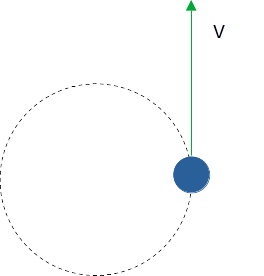
\includegraphics[scale=0.4]{UCM_vel.png}
\caption{In uniform circular motion, the instantaneous velocity is tangential (along the outside) of the circular path the object moves along.}
\label{ucm_vel}
\end{figure}

What is the acceleration of an object in uniform circular motion? The first part of answering that is figuring out the direction of the acceleration. In order for an object to move in a circular path, its velocity must be along the circle. That means the instantaneous velocity is always \textbf{tangential} to the circle, as seen in Figure \ref{ucm_vel}. 

The speed of the object is constant so the magnitude of the velocity is constant. The direction of the velocity is always changing in order to keep the velocity tangential to the circle. As we saw in Section REF HERE, we can consider perpendicular motion separately. That means that if the force is perpendicular to the velocity, it will change the direction of the velocity without changing the magnitude of the velocity. Therefore, the acceleration is directed radially toward the center of the circle, as seen in Figure \ref{ucm_accel}.

\begin{figure}[t]
\centering
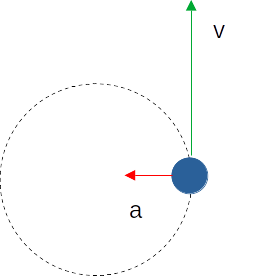
\includegraphics[scale=0.4]{UCM_accel.png}
\caption{In uniform circular motion, the instantaneous acceleration is radial, directed toward the center of the circular path the object moves along.}
\label{ucm_accel}
\end{figure}

Now to find the magnitude of the acceleration. Doing this rigorously requires calculus but we can still get some understanding of the result.

What if the velocity increases? Increasing the velocity will increase the change in velocity. If the velocity vectors are longer, then the $\Delta v$ vector will be longer as well. Since acceleration is $a_{avg} = \frac{\Delta v}{\Delta t}$, increasing $\Delta v$ will increase the acceleration. Increasing velocity will also decrease the time interval it takes for the object to travel along the path of the circle. Decreasing $\Delta t$ will increase the acceleration.

What if the radius of the circle increases? That increases the distance the object has to move for the same change in velocity $\Delta v$. If the velocity is the same, that will increase the time required. This means that increasing the radius decreases the acceleration.

We have 2 ways that increasing velocity increases acceleration and 1 way that increasing radius decreases acceleration. This would lead us to propose

\begin{equation}
a_c = \frac{v^2}{r}
\label{centaccel}
\end{equation}

as the acceleration, which is in fact exactly what we would get if we did the required calculus to solve it! This acceleration is called the \textbf{centripetal acceleration}, where centripetal means directed toward the center. That's why we denote this acceleration with a subscript $c$.

The magnitude of the acceleration is constant, so why isn't this constant acceleration motion? The answer lies in the fact that the acceleration is always directed toward the center of the circle. As the object moves around the circle, the direction of the acceleration must be constantly changing so that the acceleration is always pointed toward the center of the circle. That changing direction is why the acceleration isn't constant in uniform circular motion.

\begin{exampleblock}
Alex is jogging at $2.5 \, \frac{m}{s}$ around a circular track of radius $10.0 \, m$. What is their centripetal acceleration?

We can plug in the velocity and radius into Equation \ref{centaccel}

\begin{equation}
a_c = \frac{(2.5 \, m/s)^2}{10.0 \, m} = 0.625 \, \frac{m}{s^2}
\end{equation}

Alex has a centripetal acceleration of $a_c = 0.625 \, \frac{m}{s^2}$.
\end{exampleblock}

\begin{exampleblock}
An amusement park wants a rollercoaster to have a centripetal acceleration that is ``half a g'' ($\frac{g}{2} = 4.9 \, \frac{m}{s^2}$) while going around a circular curve. If rollercoaster is moving at a velocity of $21 \, \frac{m}{s}$ around the curve, what is the radius of the curve?

First we can start with Equation \ref{centaccel} and solve for the radius.

\begin{equation}
a_c = \frac{v^2}{r}
\end{equation}

\begin{equation}
a_c r = v^2
\end{equation}

\begin{equation}
r = \frac{v^2}{a_c} = \frac{(34 \, m/s)^2}{4.9 \, m/s^2} = 90.0 \, m
\end{equation}

The radius of the curve has to be $90.0 \, m$. (You can think of this as if the curve was extended to a full circle, that circle would have a radius of 90.0 $m$.)
\end{exampleblock}

\chapter{Forces}
\setcounter{example}{1}
\addtocounter{chp}{1}

We spent the previous chapter talking about motion, but we have yet to address the physical reason \textit{why} objects move. What is the interaction that causes motion? That is the question that will motivate this chapter.

\section{Newton's Laws of Motion}

Isaac Newton (1643 - 1727) formulated 3 laws of motion that are a major foundation of physics. His laws describe how \textbf{forces} act on objects to affect their motion. Forces can be thought of as a push or pull on an object. We will go into more detail on specific forces later, but for now we can think of them as a push or pull.

\linespace

Newton's 1st Law of Motion states that

\hspace{10pt}

\textbf{``An object in motion remains in uniform motion and an object at rest remains at rest, unless acted upon by an external force''}

\linespace

What this means that an object will remain in its current state unless an outside force acts on it. If the object is at rest, it will not start moving unless an outside force acts on it. If it is moving, it will keep moving at a constant velocity (meaning same speed and direction) unless a force acts on it.

\linespace

Newton's 2nd Law of Motion states that

\hspace{10pt}

\textbf{``The net force acting on an object is equal to the product of its mass and acceleration.''}

\begin{equation}
\overrightarrow{F_{net}} = m \overrightarrow{a}
\label{2ndlaw}
\end{equation}

\linespace

Newton's 2nd Law of Motion gives the relationship between force as an equation we can use to mathematically describe the motion. Force and acceleration both being vector quantities means that the acceleration is in the same direction as the net force.

\textbf{Net force} means the sum of all forces acting on an object. In most cases objects will have 2 or more forces acting on them, so we will need to add those forces to get the net force acting on the object.

An object's mass determines its resistance to acceleration from a force. This resistance is called \textbf{inertia}. The larger the mass, the higher the inertia, and the less an object will accelerate when acted upon by a given force.

\linespace

Newton's 3rd Law of Motion states that

\hspace{10pt}

\textbf{``When object A exerts a force on object B, object B exerts a force on object A that is equal in magnitude and opposite in direction.}

\linespace

What this means is that when one object pushes on another, the second object pushes back on the first. When the law says ``equal in magnitude'', it means that the forces are the same numerical value. If object A exerts a $5 \, Newton$ force on object B, object B exerts a $5 \, Newton$ force on object A. This is also called the \textbf{action-reaction principle}. For every force, there is an equal and opposite reaction force. The reaction force has the same strength, but is in the opposite direction.

One way you can see this for yourself is to push on a wall. What happens when you do that? You will feel like you are being pushed away from the wall! That is because when you exert a force on the wall, the wall exerts an equal and opposite force on you. 



\section{Force exerted by gravity}

In Section \ref{gravsec} we looked at the acceleration due to gravity and how it is a constant acceleration $g = 9.8 \, \frac{m}{s^2}$ for any object in free-fall. Let's apply Newton's 2nd Law of Motion free-fall. Start with \ref{2ndlaw} and plug in $g$ for the acceleration.

\begin{equation}
F_{net} = mg
\end{equation}

For an object in free fall, the net force has magnitude $mg$ direction straight down. Since the only acceleration in free-fall is due to gravity, we know that the only force acting on an object in free-fall is gravity. Therefore, we can say that the force of gravity acting on an object of mass $m$ is

\begin{equation}
F_g = mg 
\label{fg}
\end{equation}

which will always be directed straight down. This force acts on any object at the Earth's surface, even if the object is not in free-fall. Early on, we said that weight is not the same as mass. \textbf{Weight} is the force of gravity acting on an object. Weight is proportional to mass, but depends on the surface gravity. This is why astronauts weighed less on the moon, despite their mass remaining constant!

\begin{exampleblock}

Lucy has to move a box that weighs 235 $N$. What is the mass of the box in kilograms?

\hspace{10pt}

Here we will use equation \ref{fg} and solve for the mass $m$.

\begin{equation}
m = \frac{F_g}{g}
\end{equation}

The force of gravity is the weight, 235 $N$.

\begin{equation}
m = \frac{235 \, N}{9.8 \, m/s^2} = 24.0 \, kg
\end{equation}

The box has a mass of $m = 24 \, kg$.

\end{exampleblock}

We can say that free-fall is when the only force acting on an object is the gravitational force

\begin{equation}
F_{net} = F_{g}
\end{equation}

\section{Normal Force}
\label{nfsec}

Set any object on the table in front of you (pencil, book, cell phone, literally anything). Is it accelerating? No! The object set on the table is sitting stationary. That means its acceleration is zero, and from Newton's first law we know that means there is no net force acting on the object.

The force of gravity is acting down on it, so there must be a force acting upward. To determine the source of the force, we can think about why the object isn't falling down. From real life experience, we can say it is obviously the table! The table stops the object from falling by exerting an upward force on the object. The force a surface exerts on an object is called the \textbf{normal force}. This is the force that keeps the object from moving ``through'' the surface. Normal force is always perpendicular to the surface, so on a perfectly horizontal table it is direction straight up. We will denote normal force as $F_N$.

\begin{exampleblock}


A book of mass $0.40 \, kg$ is sitting stationary on a table. What is the normal force acting on the book?

\hspace{10pt}

Let's call up positive. Since the book is stationary, we know its acceleration is zero and therefore the net force is zero. The gravitational force is $F_g$ directed downward. 

\begin{equation}
F_g = -mg
\end{equation}

The normal force is directed upward to make the net force zero.

\begin{equation}
F_{net} = F_N + F_g = 0 \, N
\end{equation}

\begin{equation}
F_N = -F_g = -(-mg)
\end{equation}

\begin{equation}
F_N = (0.40 \, kg) (9.8 \, \frac{m}{s^2}) = 3.9 \, N
\end{equation}

The normal force for an object sitting on a horizontal surface with no other forces acting on it is the same as the gravitational force, just directed upward.

\end{exampleblock}

\section{Forces in 2 dimensions}

Many physical situations have forces exerted along 2 dimensions. For example, if we have a box sitting on the floor and somebody pushes it we have 3 forces acting on the box:

\begin{enumerate}
\item Gravity acting downward.
\item Normal force acting upward.
\item The person's push acting horizontally.
\end{enumerate}

This scenario has forces that act vertically and horizontally. When studying motion like this, we can take advantage of the fact that \textbf{perpendicular forces are independent}. What this means is that a vertical force acting on an object has no impact on the horizontal motion of that object. For the box being pushed along the floor, we can analyze gravity and normal force together since they are vertical forces. Then we can look at the push separately since that is horizontal.

When we have forces that aren't perfectly horizontal or vertical, we can split them into vertical and horizontal components. Figure \ref{ForceAngle} shows how a force angled at an angle $\theta$ is split into horizontal and vertical components.

\begin{figure}[H]
\centering
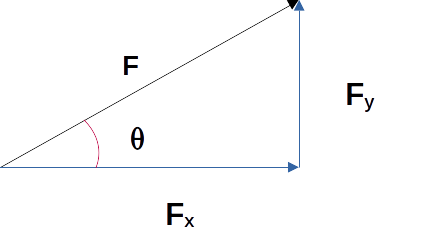
\includegraphics[scale=0.6]{Force_Angle.png}
\caption{A force directed at an angle $\theta$ above horizontal split into components. Horizontal is $F_x$ and vertical is $F_y$.}
\label{ForceAngle}
\end{figure}

You can see that the force and components form a right triangle, with the force $F$ as the hypotenuse and the components $F_x$ and $F_y$ are the legs of the right triangle. We can use \textbf{trigonometry} to find the sides. From a previous math class you should have seen the trigonometry functions sine, cosine, and tangent. They are give the relationships between the opposite leg, adjacent leg, and hypotenuse of a right triangle.

\begin{equation}
sin(\theta) = \frac{opposite}{hypotenuse}
\end{equation}

\begin{equation}
cos(\theta) = \frac{adjacent}{hypotenuse}
\end{equation}

\begin{equation}
tan(\theta) = \frac{opposite}{adjacent}
\end{equation}

From the angle $\theta$ the horizontal component is the adjacent side, so we can find $F_x$ as

\begin{equation}
F_x = F \, cos(\theta)
\end{equation}

The vertical component is the opposite side of the triangle, so we can find $F_y$ as

\begin{equation}
F_y = F \, sin(\theta)
\end{equation}

\section{Free Body Diagrams}

If we return to looking at a book on the table, we looked at a situation where there are multiple forces acting in different directions on an object. This can be difficult to keep track of as just text, so in these cases we draw pictures known as \textbf{free body diagrams}. These diagrams are simple pictures that show the forces acting on one object. The forces are drawn as arrows in the direction of the force, with the relative length of the arrows in the free body diagram showing the relative magnitudes of the forces. The free body diagram for a book sitting stationary on a table is:

FBD HERE

\section{Friction}

What happens if you slide a book across a table? It will slow down and eventually stop. From Newton's 1st Law of Motion, the change in velocity means there must be a net force. This net force is supplied by \textbf{friction}, which is the resistance to 2 surfaces sliding against each other. There are 2 types of friction:

\begin{enumerate}
\item \textbf{Kinetic friction} - acts when surfaces are sliding against each other. Slows down the moving object(s).

\item \textbf{Static friciton} - acts when the surfaces are stationary relative to each other. Acts to prevent the surfaces from moving.
\end{enumerate}

Different surfaces will have different friction forces. We know that a hockey puck will slide further on ice than on carpet before stopping, so there is a characteristic of the surfaces that determines the force. The surface interactions are described by the \textbf{coefficient of kinetic friction} and \textbf{coefficient of static friction}. In equations we will denote these coefficients with the Greek letter $\mu$, pronounced ``mu''. Subscripts are used to differentiate kinetic friction $\mu_k$ from static friction $\mu_s$. The force of kinetic friction is found by

\begin{equation}
F_k = \mu_k F_N
\label{kfriction}
\end{equation}

which is the normal force multiplied by the coefficient of kinetic friction. This means that if the coefficient of kinetic friction or the normal force increases, the force of kinetic friction increases.

\begin{exampleblock}

A box of mass $30.0 \, kg$ is sliding along a horizontal floor. The coefficient of kinetic friction between the floor and box is $\mu_k = 0.40$. What is the magnitude of kinetic friction acting on the box?

\hspace{10pt}

The normal force here can be found by looking at the vertical axis. The box is not moving up or down, so the gravitational force and normal force are equal in magnitude.

\begin{equation}
F_N = F_g = mg = (30.0 \, kg)(9.8 \, \frac{m}{s^2} = 294 \, N
\end{equation}

The force of kinetic friction is then

\begin{equation}
F_k = \mu_k F_N = 0.40 \cdot (294 \, N) = 118 \, N
\end{equation}

The force of kinetic friction on the box is $F_k = 118 \, N$

\end{exampleblock}

Notice how the coefficient of kinetic friction has no units. That is because it is multiplied by a force to find a force. It is a dimensionless (unitless) factor describing how the 2 surfaces interact when sliding along each other.

The force exerted by static friction is found by

\begin{equation}
F_s \leq \mu_s F_N
\label{sfriction}
\end{equation}

This is very similar to the force of kinetic friction, except that the coefficient is switched out for the coefficient of static friction. However, there is one major difference: \textit{the equal sign is replaced with a less than or equal sign}. That is because static friction prevents an object from starting to slide, and will not cause one surface to slide past another. In terms of Newton's Laws of Motion, static friction opposes an applied force to make the net force zero. If the applied force is larger than $\mu_s F_N$, then the static friction force is cannot make the net force zero and the object will begin sliding. 

\begin{exampleblock}

A paperweight of mass $0.75 \, kg$ is sitting on a desk. The coefficient of static friction between the desk and paperweight is $\mu_s = 0.54$. There is a force of $3.0 \, N$ pushing horizontally on the paperweight, trying to slide it on the desk. Does the paperweight slide on the desk? If not, what is the magnitude of the static friction force acting on the paperweight?

\hspace{10pt}

First we need to find out the maximum possible static friction force. First we find the normal force, which is equal to the gravitational force.

\begin{equation}
F_N = F_g = (0.75 \, kg) (9.8 \, \frac{m}{s^2}) = 7.35 \, N
\end{equation}

Now we can use Equation \ref{sfriction} to find the static friction force.

\begin{equation}
F_s \leq \mu_s F_N = 0.54 \cdot 7.35 \, N = 3.97 \, N
\end{equation}

The static friction force is less than or equal to $3.97 \, N$. This means that $3.97 \, N$ is the maximum possible static friction force. Since the applied force of $3.0 \, N$ is less than that, the static friction force can match the applied force and keep the block still.

Now to find the static friction force, we need to find the force required so that the net force is zero. 

\begin{equation}
F_{net} = F_{app} + F_s = 0
\end{equation}

If we say the applied force ($F_{app}$) is in the positive direction, we can solve the problem as such

\begin{equation}
F_s = -F_{app} = - 3.0 \, N
\end{equation}

The force of static friction is $F_s = 3.0 \, N$ in the opposite direction of the applied force. Note that $F_s$ is not always equal to $mu_s F_N$!

\end{exampleblock}



\chapter{Work, Energy, and Power}
\setcounter{example}{1}
\addtocounter{chp}{1}

\end{document}
